\section{Подсчет задачи на примерах из жизни}\label{examples}

Варианты с разными параметрами. Подставим некоторые реальные данные:

\subsection{СК <<Олимпийский>> (Москва)}

\begin{itemize}
	\item Количество парковочных мест: $700$ \footnote{Источник: https://carparkings.ru/parkovki/moskva/parkovka-u-sportivnogo-kompleksa-olimpijskij.html}.
	\item Максимальная вместимость: $35 000$ зрителей
	\item Максимальная вместимость после реставрации: $10 000$ \footnote{Источник: https://ru.wikipedia.org/wiki/Олимпийский}
\end{itemize}
$0,02$ в старой конфигурации
$0,07$ после реставрации

\subsection{Крокус Сити холл (Москва)}
\begin{itemize}
	\item Максимальная вместимость зала: $7233$
	\item Парковка $6000$ \footnote{Источник: https://crokus-hall.com/about/}
\end{itemize}

$0,83$

\subsection{Альберт-холл (Лондон)}

\subsection{Москва-сити}
\begin{itemize}
	\item Количество парковочных мест $10 500$  \footnote{Источник: http://moscow-city-towers.ru/parking.php}
	\item Посещаемость в день:  $175 000$ \footnote{Источник: https://moscow-city.online/news/34113/}
\end{itemize}

0,06

\subsection{Филармония (г. Майкоп)}
%\footnote{Предположим, что в Майкоп приехал Николай Басков, и все билеты раскуплены}

\begin{itemize}
	\item Мест в партере: $612$ \footnote{Источник: http://filarmoniya-ra.ru/interiors}
	\item Мест на парковке: $48$ \small{(посчитано по спутниковой карте)}
\end{itemize}
\begin{figure}
	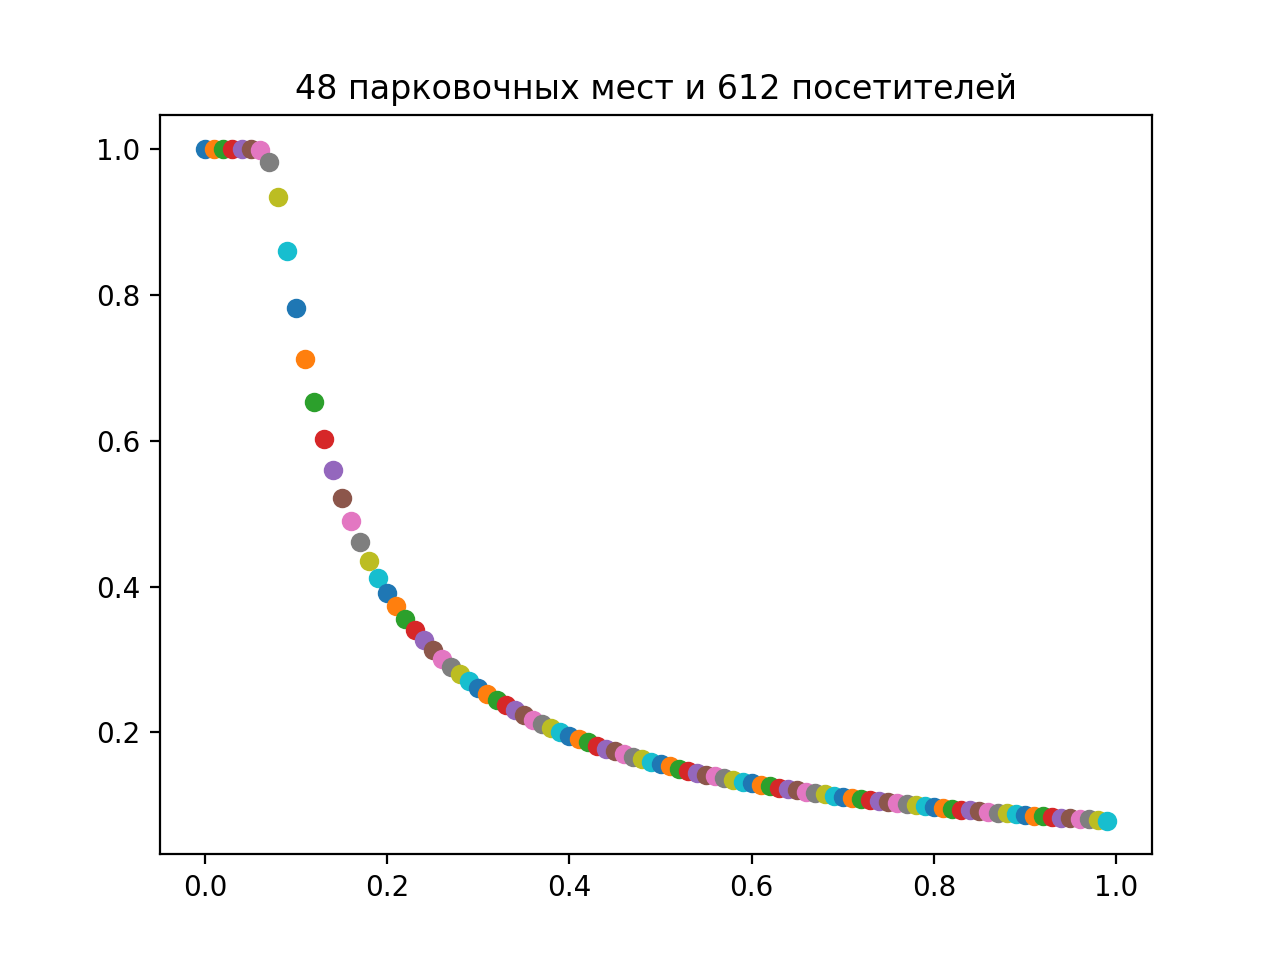
\includegraphics[scale=0.6]{img/612_48}	
\end{figure}

\begin{figure}
	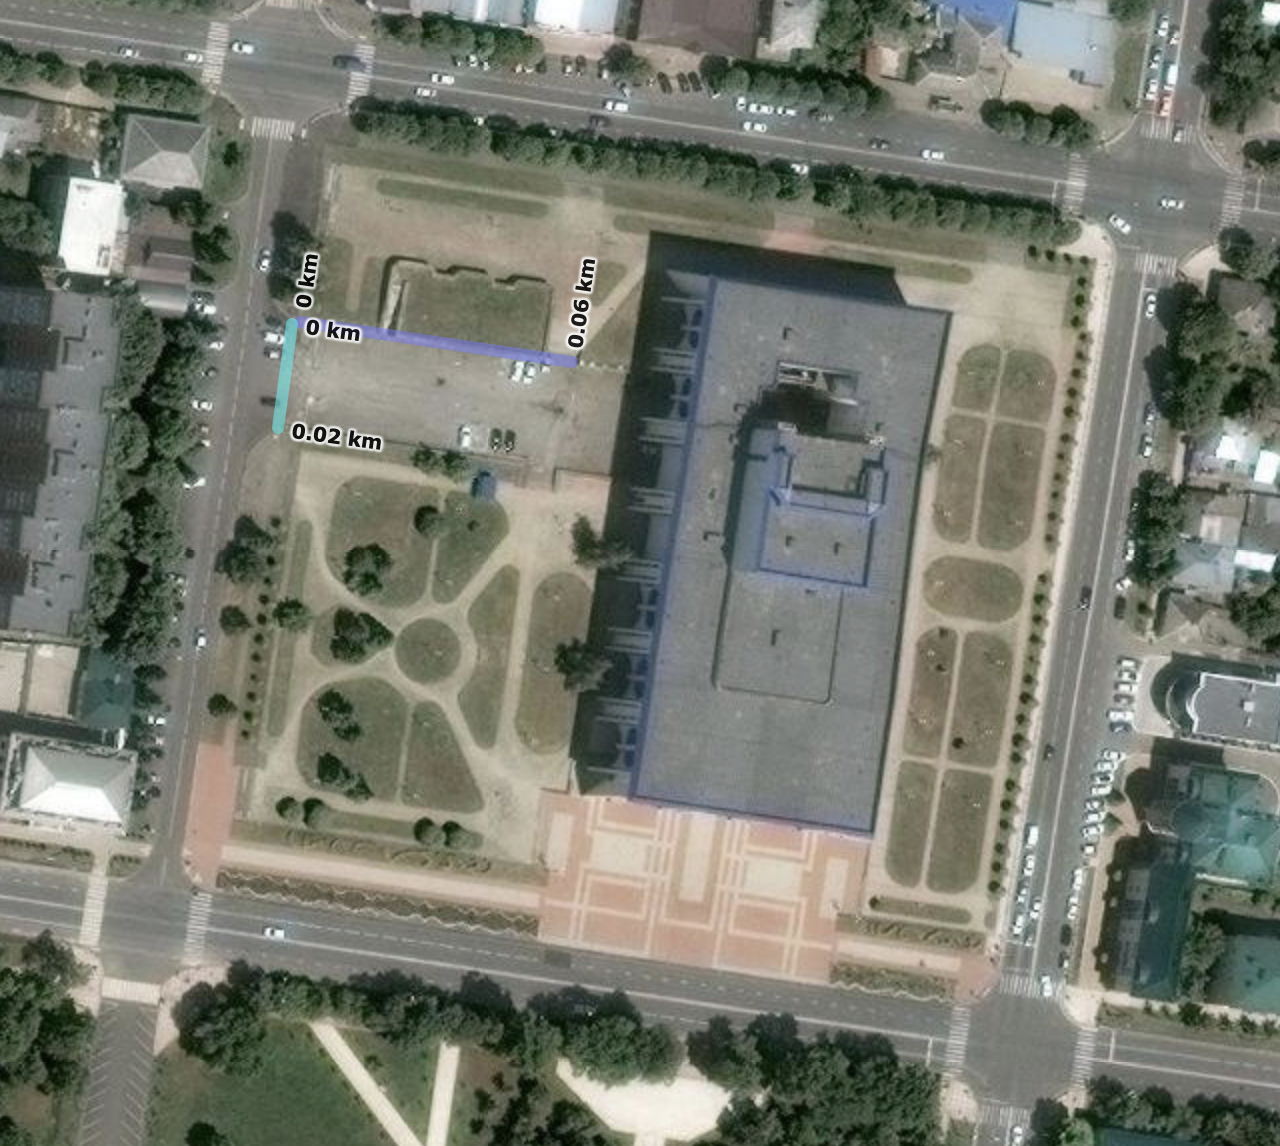
\includegraphics[scale=0.3]{img/filarmony_parking}
	\caption{Майкопская филармония на спутниковых Яндекс-картах}
\end{figure}

0,07

